\chapter{基礎知識と環境構築}

この章ではWebの中核をなすLAMPと呼ばれる概念を説明しながら、環境構築を行います。

\section{LAMPとは}

LAMPとはWebアプリケーションを作成する上で使われる、「Linux、Apache、MySQL、PHP」の四つをまとめたワードです。いまではApacheがNginxになったり、MySQLがPostgreSQLになったり、PHPがRubyだったりPythonになったりしますが、基本的な構成要素は大きく変わっていません。

\begin{center}
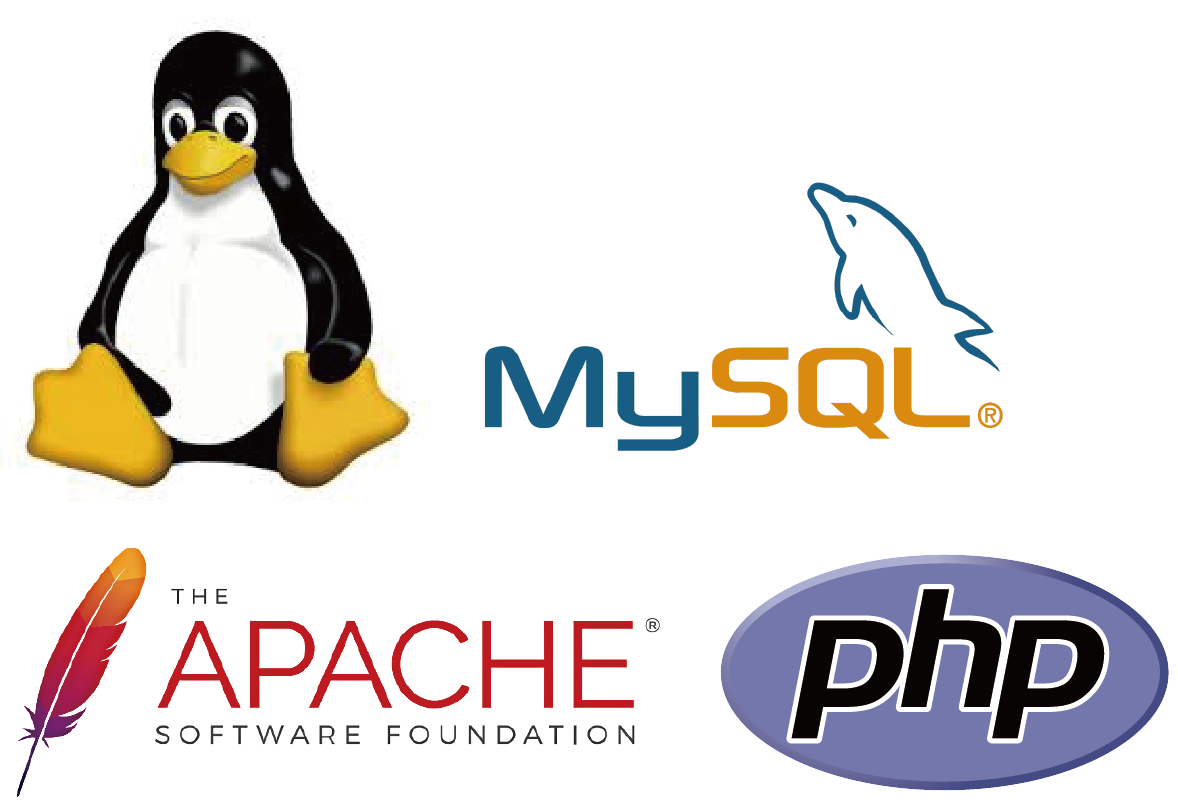
\includegraphics[width=10cm]{./chap1_fig/LAMP.png}

LAMPのそれぞれのソフトウェアのロゴ
\end{center}

\subsection{避けては通れないOS、Linux}

いまこの教材を読んでいるあなたはおそらく何らかのOSが載っているデバイスを使っていることでしょう。WindowsだったりMacOSであったりAndroidだったりするでしょう。もしプログラミングを真面目にやっていくならば、Linuxは避けては通れないOSです。LinuxはLinus TorvaldsがUNIXと呼ばれるOSをベースに開発されたOSです。オープンソースでプログラムの中身が公開されており、使用するのにお金がかからないので多くの電子機器で利用されています。先ほど述べたAndroidもLinuxをベースに作られています。DockerはLinuxの上で動作しますし、組み込みでもLinuxが標準的なOSになりつつあります。Linuxを避けてプログラミングをするのはもう難しいでしょう。

\subsection{WebサーバーのApache}

Webサーバーです。インターネットでの情報はバケツリレーです。自分勝手にデータを投げつけてもだれも回してくれません。どのように接続を確立してどんな形でデータを送るかの約束事を「プロトコル」と言います。Webサービスにおいては、HTTPと呼ばれるプロトコルでデータを送受信します。最近ではデータを暗号化して、バケツリレーの途中でデータが盗まれないようにしたHTTPSがよく用いられています。Apacheはこのようなプロトコルから暗号化されたデータを復号したり、取り出したデータをPHPに渡す役割をしています。

また、最近ではNginxと呼ばれるWebサーバーが用いられるようになりました。Apacheと違い、送られたデータを別の場所に中継するリバースプロキシや、送られたデータを二台以上のサーバーに分散させるロードバランサーといった機能が搭載されています。

\subsection{データベースのMySQL}

やっぱりデータを保存できなければ面白くありません。自分のツイートしかみれないTwitterは面白くないですよね?ユーザーから送信されたデータを保存するために使われるソフトウェアがデータベースです。もちろんデータをテキストファイルに保存しても問題ありません。しかし、ある日付だけ取り出したいだとか、もしコンピューターが一台壊れてもデータが消えないようにしたいだとか、そういうことを考えると全部自分でシステムをくみ上げるのは途方もない作業になります。そこでデータベースにデータを保存しておくことで、このような問題を解決します。データベースは自分の書いたプログラムからSQLと呼ばれる言語で命令を送って操作します。SQLの命令はPHPで作ってもPythonで作っても全く同じようにデータベースは動作します。なので、PHPでwebサービスを動かしながら、裏でPythonを使ってデータ分析をする、みたいな使い方をすることもできます。

\subsection{プログラミング言語のPHP}

これから学んでいくプログラミング言語です。以下の特徴があります。

\begin{itemize}
  \item HTMLに埋め込むような書き方ができる
  \item 動的型付け言語
  \item Webアプリ向けの豊富な組み込み関数
  \item Webアプリを作るうえで使われるフレームワークが豊富
\end{itemize}

\section{環境構築}

さて、これから最も難しいとされる環境構築です。


